\section{System Design and Deployment Methodology}
\label{sec:arch}

This section describes the proposed Data Platform: its cloud infrastructure, the
open-source software stack it deploys, the three-phase automated provisioning
workflow, and the configurable installation profiles that tailor the platform to
different workload types.

%%%%%%%%%%%%%%%%%%%%%%%%%%%%%%%%%%%%%%%%%%%%%%%%%%%%%%%%%%%%%%%%%%%%%%%%%%%%%%%%%%%%%%%%%%%%%%%%%%%%%%%%%%%%%%%%%%%
\subsection{Cloud Infrastructure and Network Topology}

The infrastructure runs on Oracle Cloud Infrastructure (OCI), using ARM-based
Ampere A1 Flex instances available through the OCI Free Tier. The cluster
consists of four virtual machines, one master node and three worker
nodes, hosted within a single subnet of an OCI tenancy
(Figure~\ref{fig:topology}). Each node is a \texttt{VM.Standard.A1.Flex}
instance with 1~OCPU (ARMv8) and 6~GB of RAM, yielding a total cluster capacity
of 4~OCPUs and 24~GB of RAM. The instances run CentOS Stream~9 on the aarch64
architecture. Persistent block volumes are attached to each instance for HDFS
data and log storage.

A security list associated with the subnet restricts external access to a
pre-defined set of IP addresses, opened through the tenancy's Internet Gateway
for the specific TCP ports required by the active installation profile (e.g.\
Ambari web UI, Spark History Server, Hive JDBC). Within the subnet, all four
nodes communicate freely over private addresses, which Apache Ambari maps during
the cluster bootstrap to assign service roles and verify host reachability.

\begin{figure}[htbp]
    \centering
    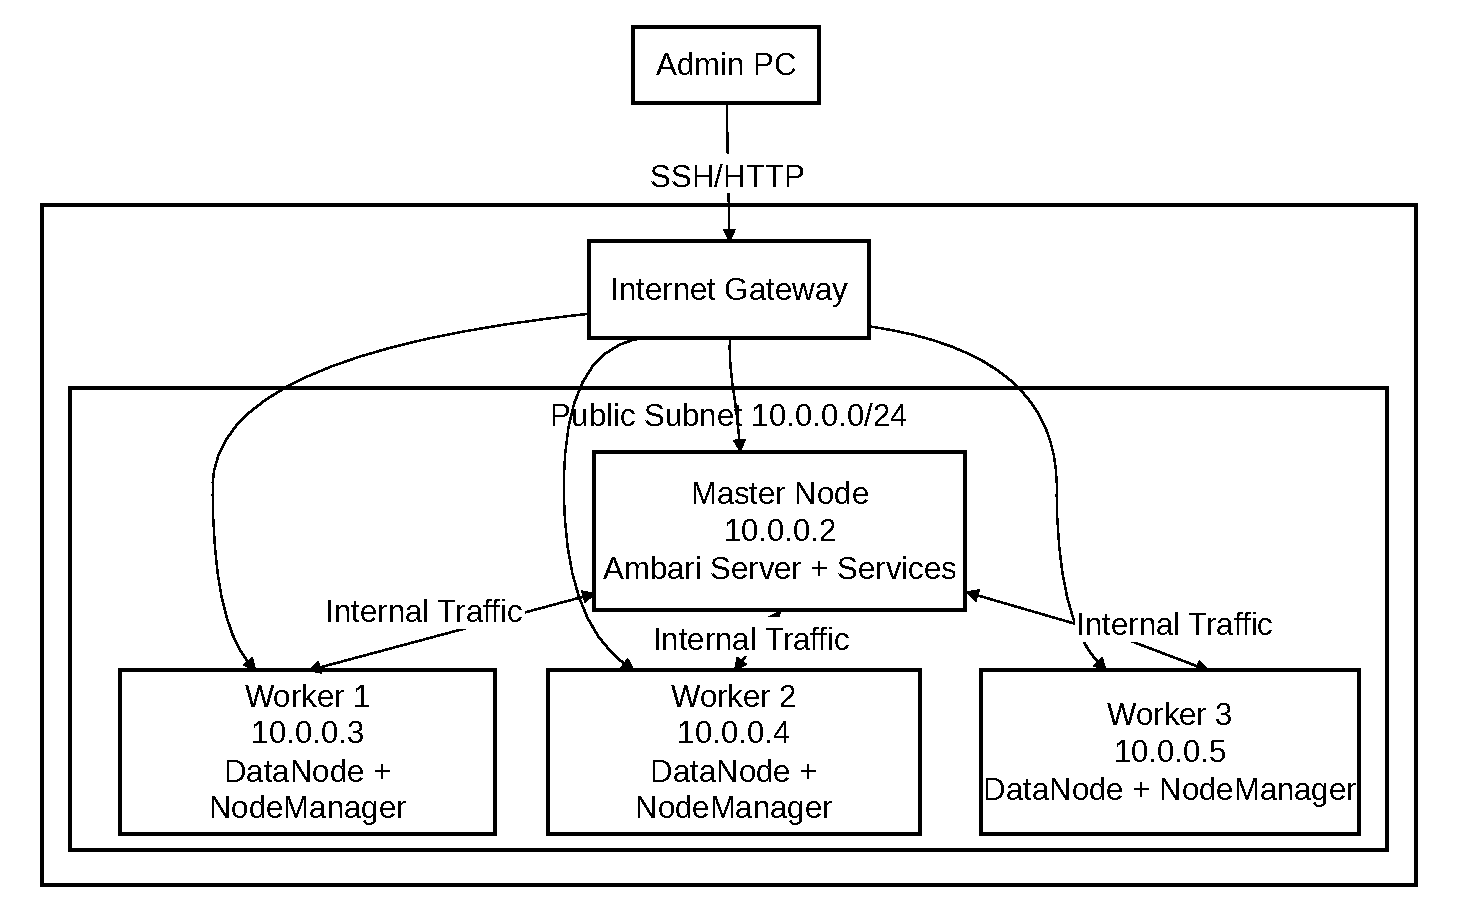
\includegraphics[width=0.9\linewidth]{content/assets/topology.pdf}
    \caption{Network topology of the four-node cluster on OCI.}
    \label{fig:topology}
\end{figure}

%%%%%%%%%%%%%%%%%%%%%%%%%%%%%%%%%%%%%%%%%%%%%%%%%%%%%%%%%%%%%%%%%%%%%%%%%%%%%%%%%%%%%%%%%%%%%%%%%%%%%%%%%%%%%%%%%%%
\subsection{Automated Deployment Workflow}

Deployment is fully automated through Infrastructure as Code and proceeds in
three sequential phases, illustrated in
Figures~\ref{fig:prov-terraform}--\ref{fig:prov-cluster}.

\paragraph{Phase~1: Terraform provisioning.}
The user configures a small set of Terraform variables, the permitted IP range
and the desired installation profile, and executes \texttt{terraform apply}.
Terraform then generates a TLS RSA key pair, provisions the network layer
(Virtual Cloud Network, subnet, security list, and Internet Gateway), and
creates the four compute instances. Ansible playbooks and Ambari API interaction
scripts are uploaded to the master node's temporary directory as part of this
phase (Figure~\ref{fig:prov-terraform}).

\begin{figure}[htbp]
  \centering
  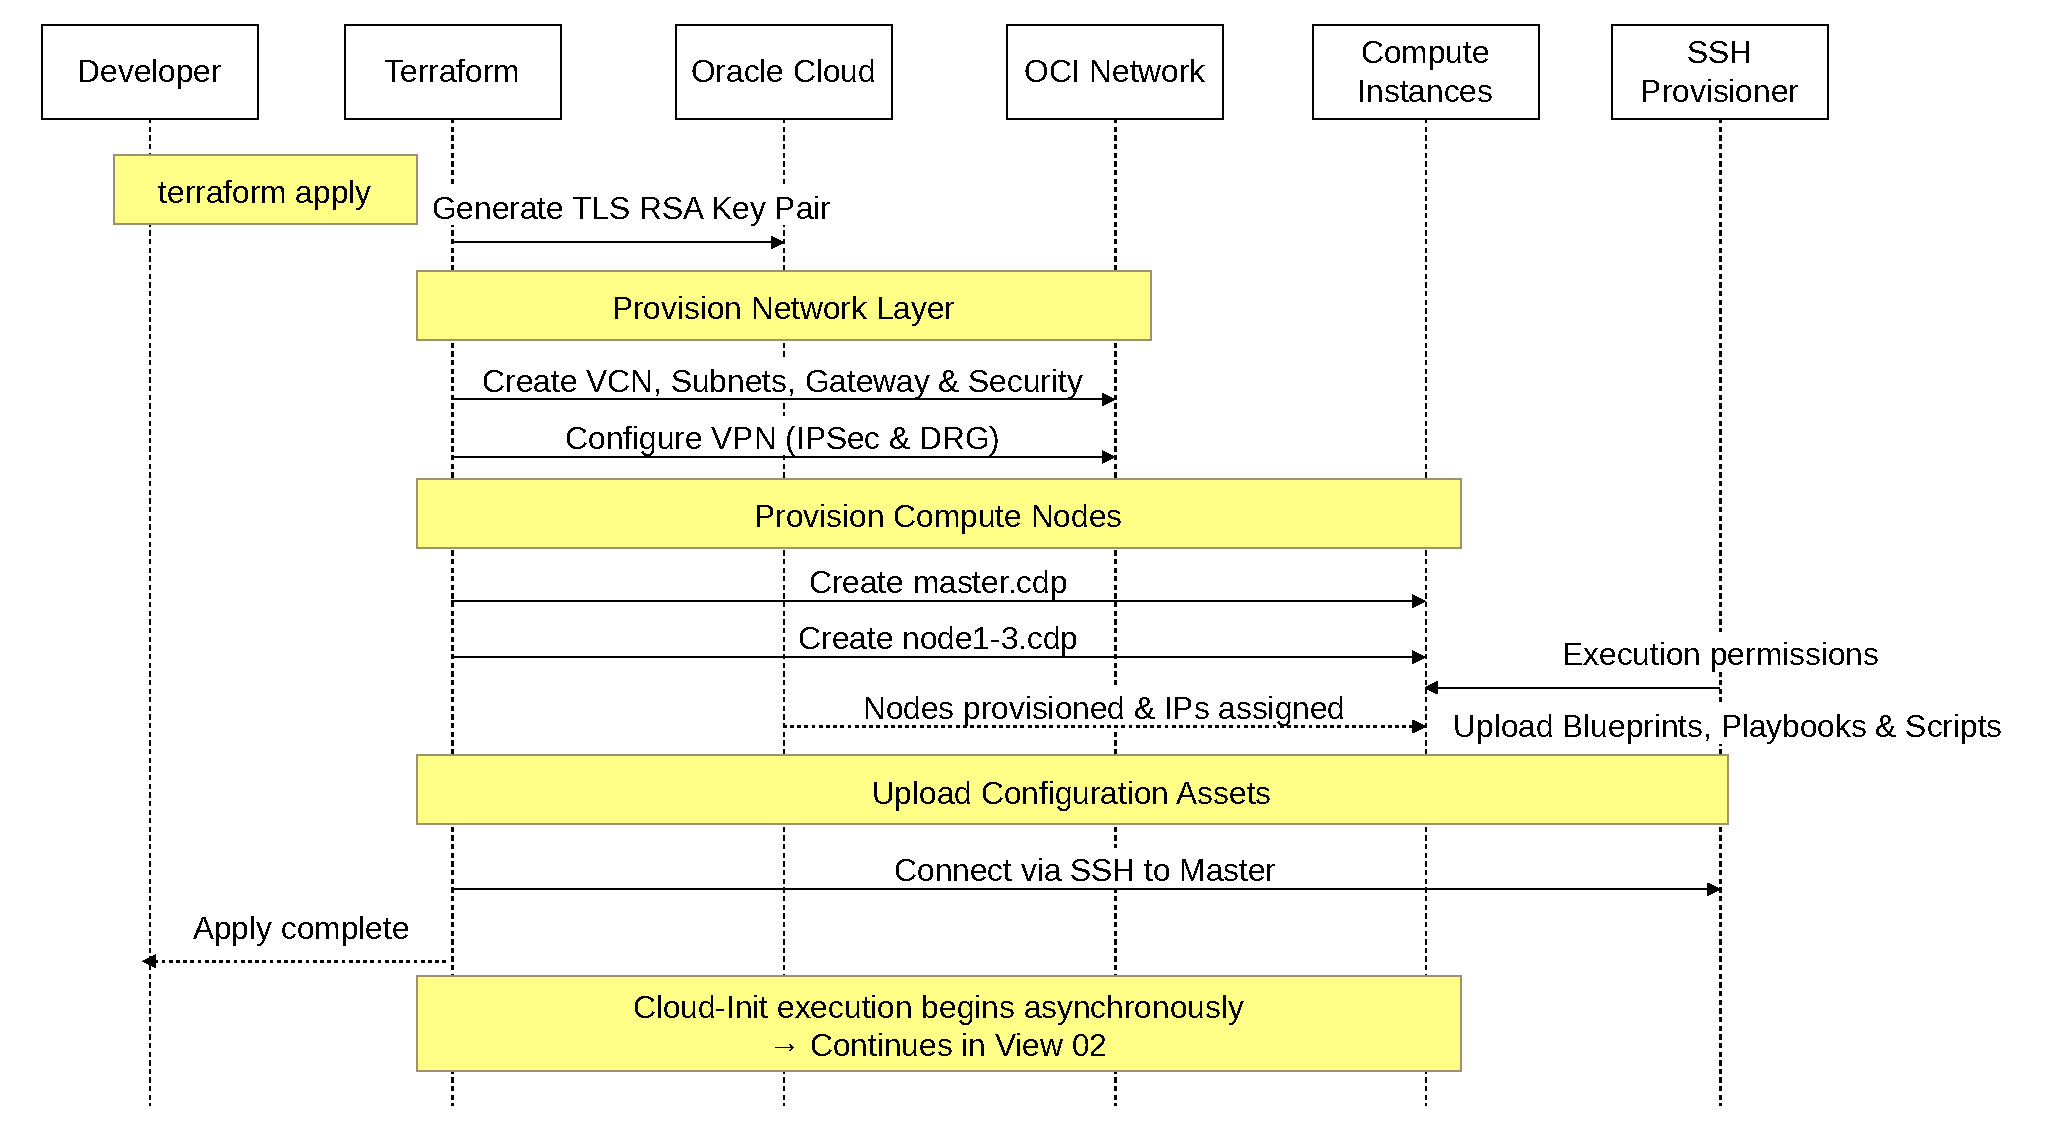
\includegraphics[width=\linewidth]{content/assets/provisioning-01-terraform.pdf}
  \caption{Provisioning workflow, Phase~1: Terraform execution sequence.}
  \label{fig:prov-terraform}
\end{figure}

\paragraph{Phase~2: OS-level configuration.}
On first boot, a \texttt{cloud-init} script on the master node installs Python
and Ansible, configures host resolution via \texttt{/etc/hosts} on all nodes,
and applies baseline OS security rules (Figure~\ref{fig:prov-os}). Ansible is
installed only on the master, which orchestrates the remaining configuration
through SSH connections to each worker. The \texttt{site.yml} playbook installs
prerequisite packages, notably OpenJDK~1.8 as the JVM runtime for all Hadoop
services and chrony for NTP-based clock synchronisation across the
cluster, initialises the PostgreSQL-backed Ambari database schemas, and deploys
the Ambari Server on the master and Ambari Agents on all four nodes. At this
point the cluster is ready to receive the application-level deployment
orchestrated by Ambari.

\paragraph{Phase~3: Ambari-driven cluster deployment.}
Once the Ambari infrastructure is running, a shell script on the master node
registers the application blueprint via the Ambari REST API. The blueprint is a
JSON document that maps each Hadoop component to its designated node role
(e.g.\ DataNode, NodeManager) according to the selected installation profile;
it also encodes service-level configurations such as the HDFS replication
factor, YARN scheduler settings, and Hive Metastore connection parameters. The
script then submits a cluster-creation request that references the registered
blueprint and a host-mapping template (Figure~\ref{fig:prov-cluster}).

During this phase, Ambari downloads the ODP~1.2.2.0 RPM packages from an
external repository, installs them on each node, and starts the services in
dependency order. The deployment incorporates an automated recovery engine: if
Ambari reports a failure at any stage, the engine stops the Ambari Server,
clears HDFS and HBase state directories, resets the PostgreSQL database, and
restarts the server, retrying the full deployment up to three times. If all
retries are exhausted, a manual initialisation script is available as a
fallback. The end-to-end process, including potential recovery cycles and the
retrieval of external component binaries, takes approximately three hours on the
Free Tier network bandwidth.

\begin{figure}[htbp]
  \centering
  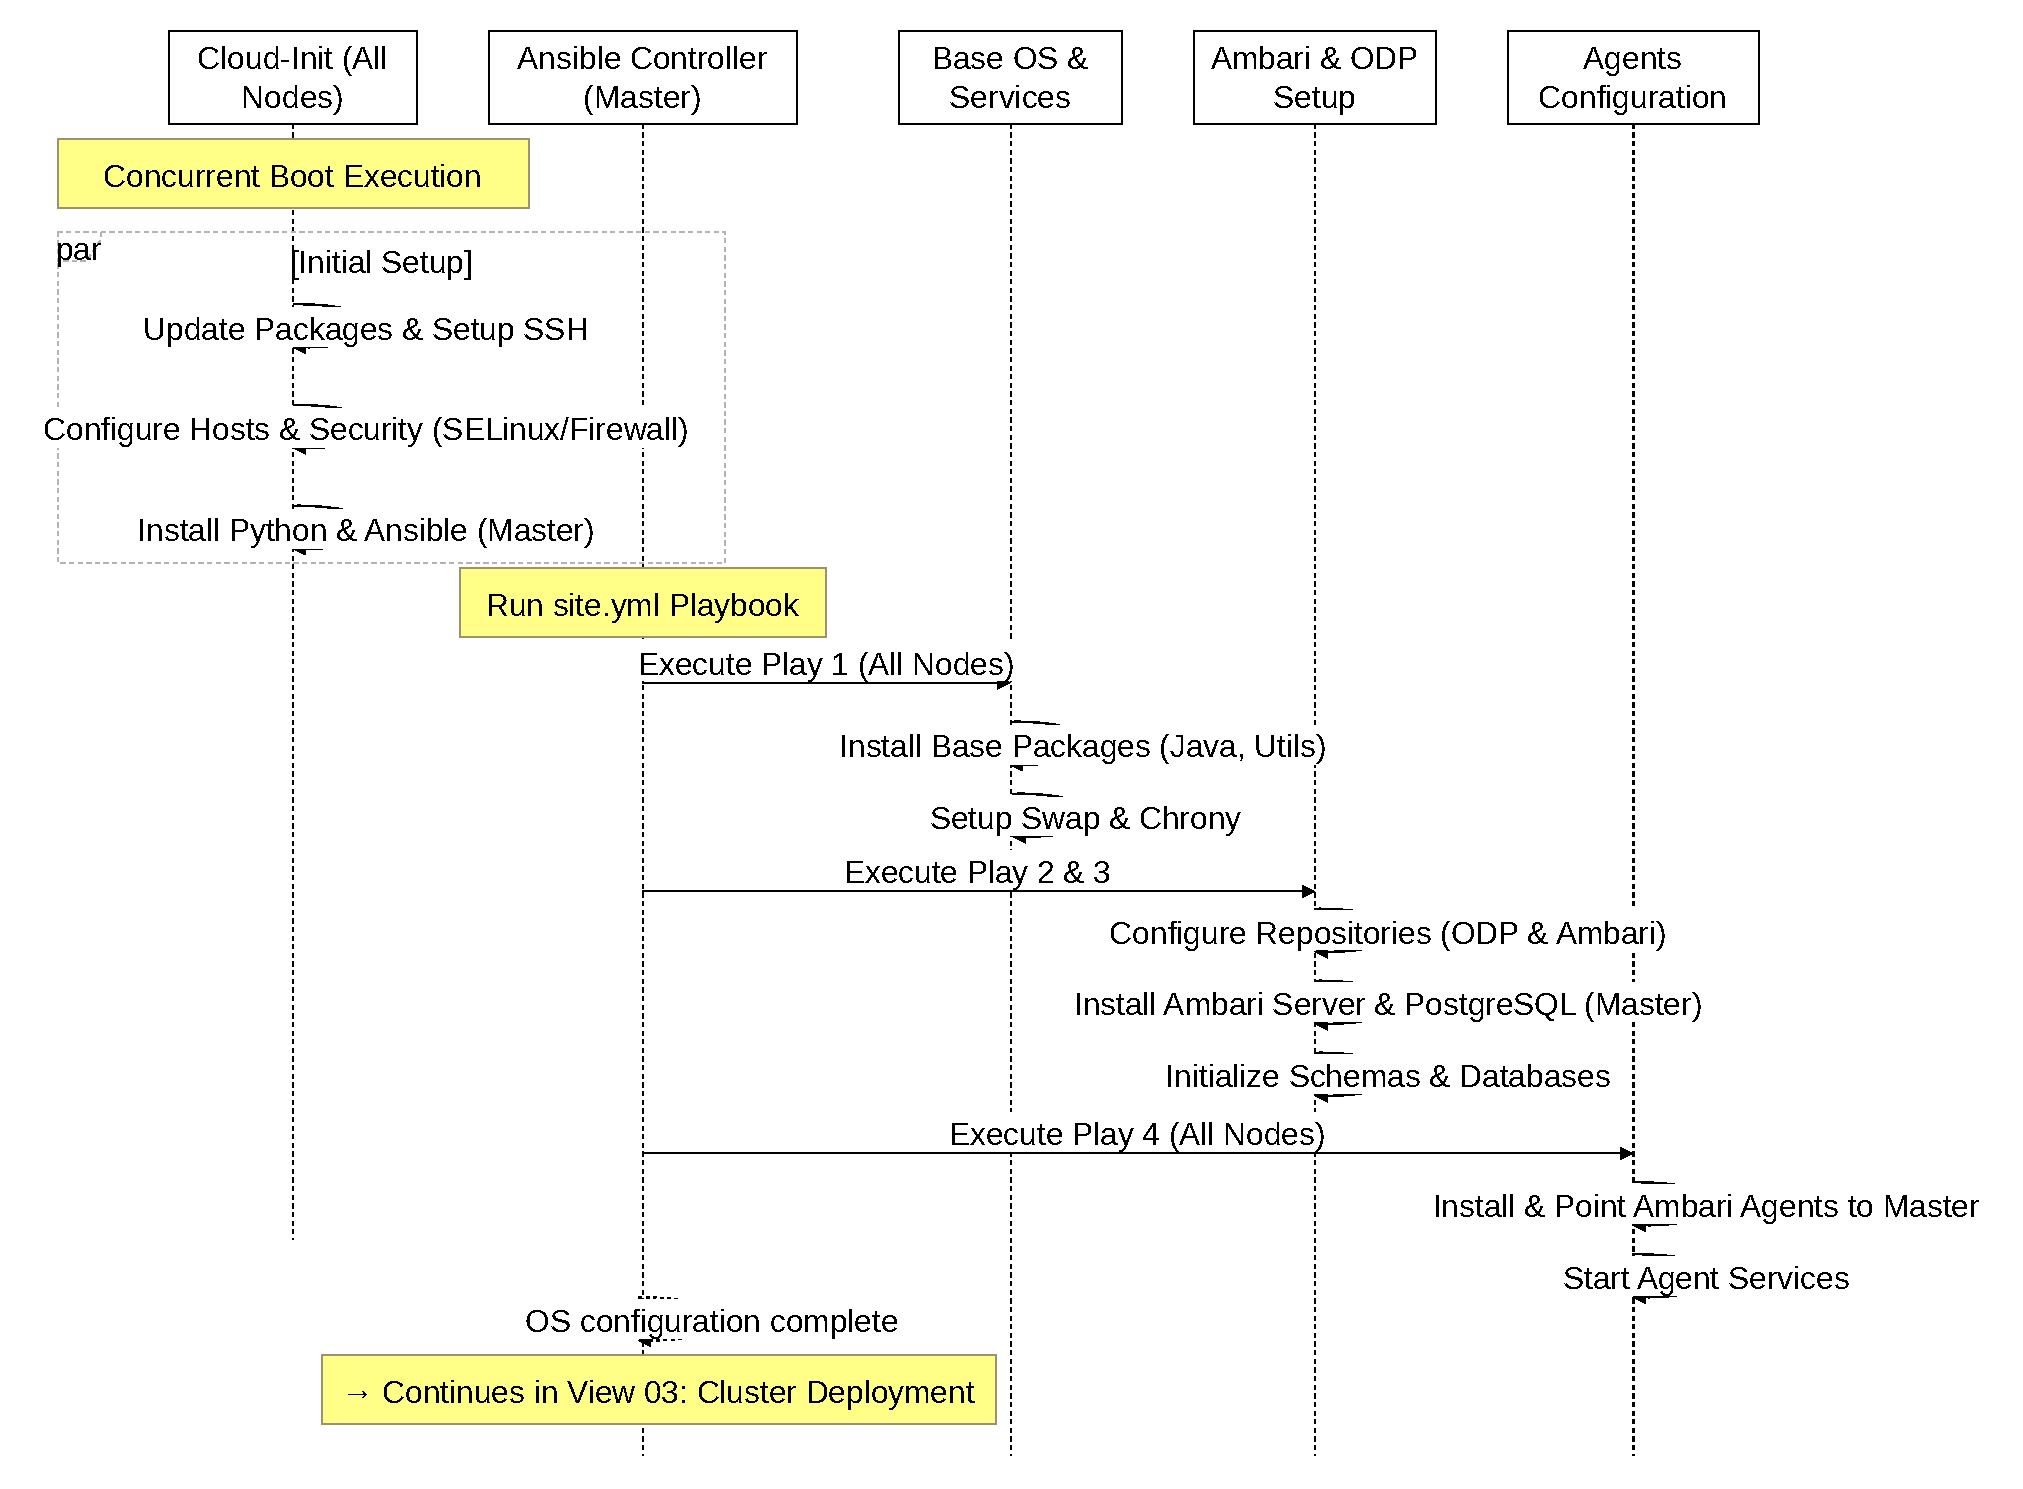
\includegraphics[width=1.0\linewidth,height=0.36\textheight,keepaspectratio]{content/assets/provisioning-02-os.pdf}
  \caption{Provisioning workflow, Phase~2: OS-level configuration via cloud-init and Ansible.}
  \label{fig:prov-os}

  \vspace{0.6cm}

  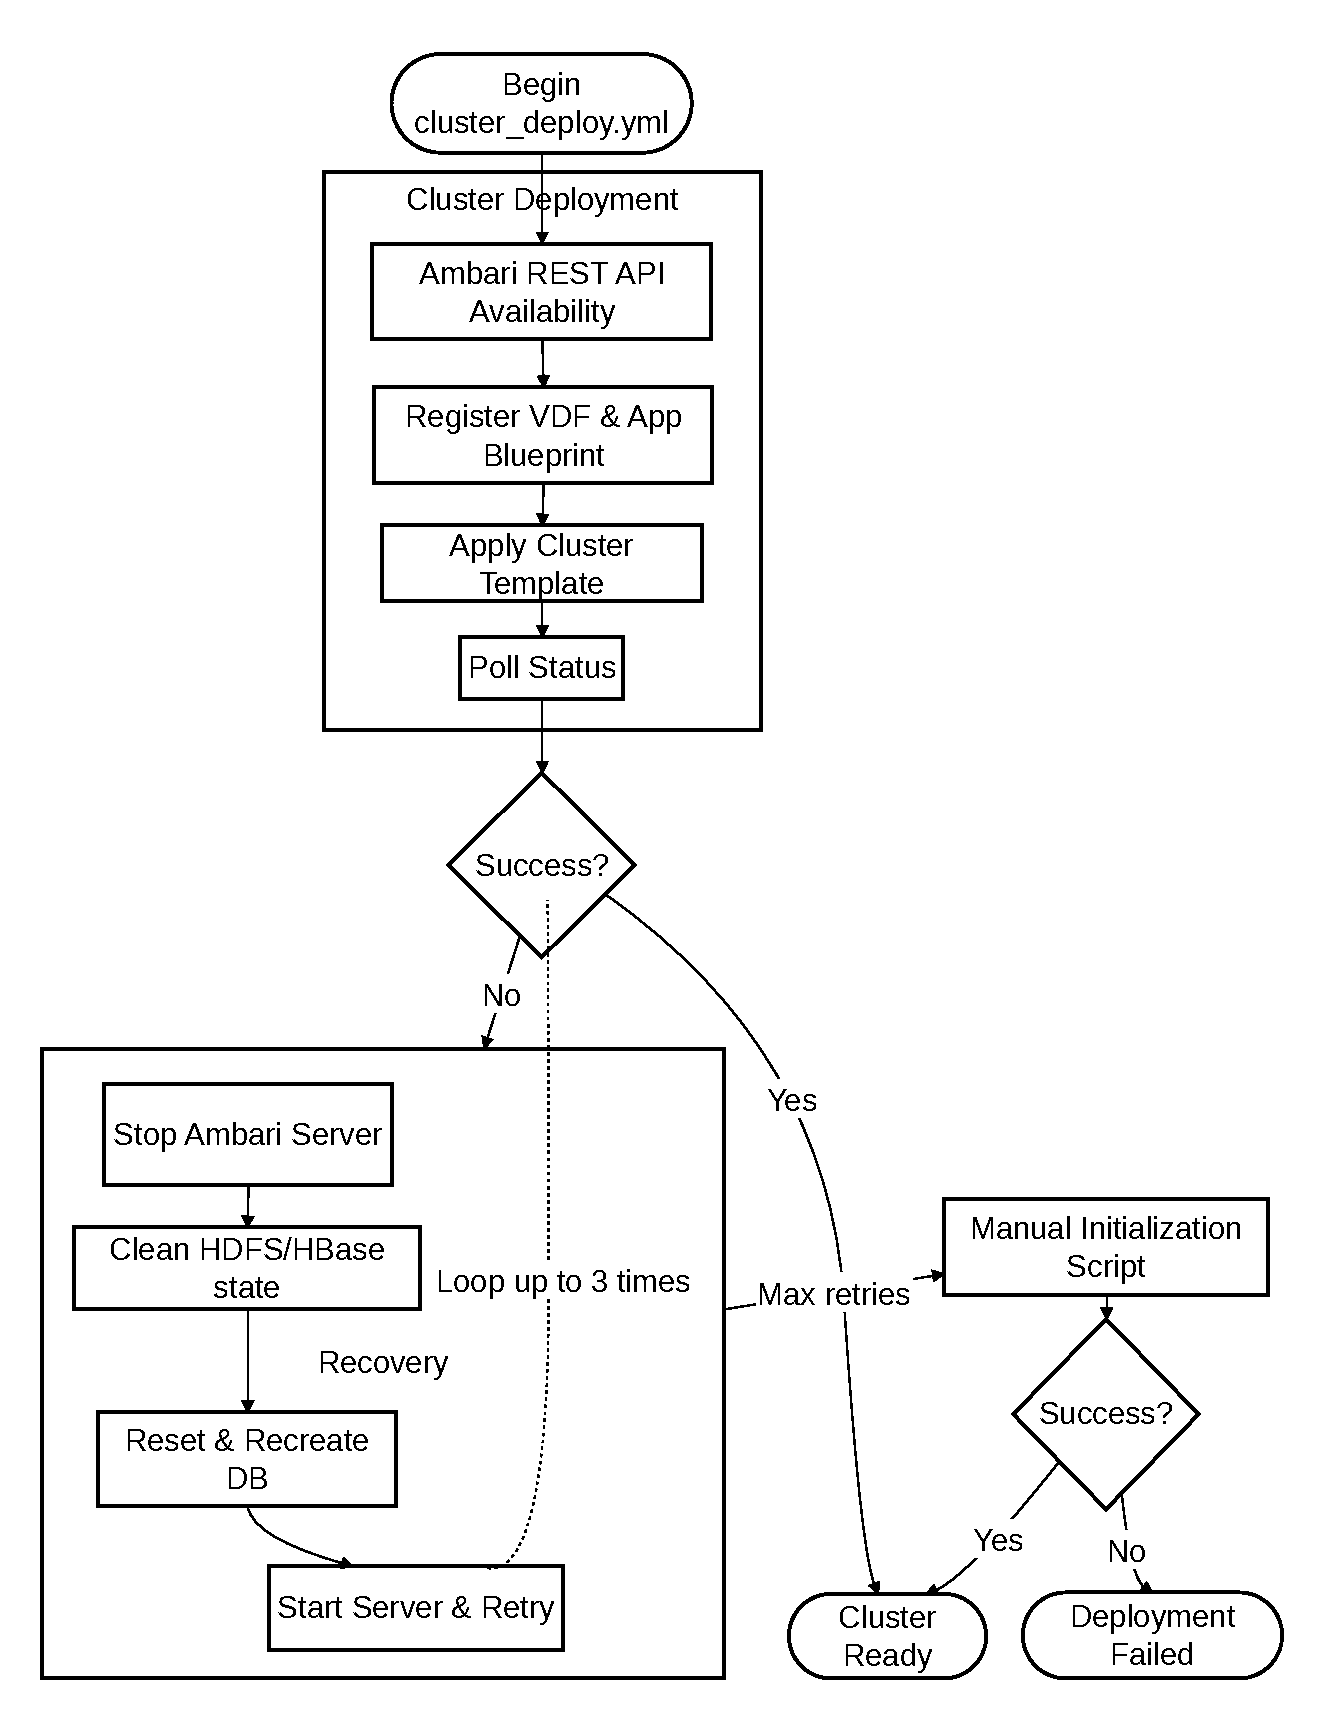
\includegraphics[width=1.0\linewidth,height=0.36\textheight,keepaspectratio]{content/assets/provisioning-03-cluster.pdf}
  \caption{Provisioning workflow, Phase~3: Ambari REST API cluster deployment with recovery logic.}
  \label{fig:prov-cluster}
\end{figure}

%%%%%%%%%%%%%%%%%%%%%%%%%%%%%%%%%%%%%%%%%%%%%%%%%%%%%%%%%%%%%%%%%%%%%%%%%%%%%%%%%%%%%%%%%%%%%%%%%%%%%%%%%%%%%%%%%%%
\subsection{Data Lake Architecture}

The resulting environment is organised into four functional layers, depicted in
Figure~\ref{fig:arch-default}. The software stack is built on version~1.2.2.0
of the OpenSource Data Platform (ODP) \citep{clemlab_odp_docs_intro_1310},
managed by Apache Ambari. ODP distributes its components as native aarch64 RPM
packages for CentOS Stream~9, ensuring that every service in the Hadoop
ecosystem executes natively on the ARM Ampere A1 instances without
cross-compilation or emulation. Table~\ref{tab:odp-versions} lists the
principal component versions deployed in this study.

\begin{table}[htbp]
  \centering
  \caption{Software component versions (ODP~1.2.2.0).}
  \label{tab:odp-versions}
  \renewcommand{\arraystretch}{1.2}
  \begin{tabular}{@{} l l @{}}
    \hline
    \textbf{Component} & \textbf{Version} \\
    \hline
    Hadoop (HDFS, YARN, MapReduce2) & 3.3.6 \\
    Apache Spark~3               & 3.4.2 \\
    Apache Hive                  & 3.1.3 \\
    Apache Tez                   & 0.10.2 \\
    Apache HBase                 & 2.5.6 \\
    Apache Kafka                 & 2.8.1 \\
    Apache NiFi                  & 1.24.0 \\
    Apache Ranger                & 2.4.0 \\
    Apache ZooKeeper             & 3.8.3 \\
    Java Runtime                 & OpenJDK~1.8 \\
    \hline
  \end{tabular}
\end{table}

\paragraph{Ingestion.} Apache Kafka handles real-time event streaming, decoupling
data producers from consumers to support high-throughput workloads. Apache NiFi
manages flow-based data routing with built-in back-pressure control, data
provenance tracking, and a visual pipeline editor. An NFS Gateway provides a
POSIX-compatible mount point for batch file ingestion, allowing external systems
to write data directly into HDFS without requiring Hadoop client libraries.

\paragraph{Storage.} HDFS provides block-based, replicated storage for raw and
columnar data. Files are split into blocks (128~MB by default) and replicated
across the three DataNodes for fault tolerance. Apache HBase offers low-latency
NoSQL access for random read/write workloads. The Hive Metastore maintains
schema and structural metadata for tables registered across the platform,
enabling both Hive and Spark to share a common catalogue of table definitions.

\paragraph{Processing.} Apache YARN schedules cluster resources by allocating
containers to processing engines according to the capacity available on each
NodeManager. Apache Spark~3 performs in-memory analytics and is the primary
engine for the benchmark workloads evaluated in this study. Apache Tez provides
an alternative DAG-based execution engine used by Hive for optimised query
plans. Hive Server~2 exposes an SQL interface over HDFS-resident data, serving
as the entry point for business-intelligence tools and the Beeline CLI. The
Phoenix Query Server enables SQL access over HBase tables. Spark~3 includes
Livy for REST-based remote job submission.

\paragraph{Governance.} Apache Ranger enforces role-based access control (RBAC)
and data-masking policies across all services in the stack; its audit logs are
indexed by Infra Solr for structured search and compliance reporting. Apache
ZooKeeper provides distributed coordination and leader election, ensuring that
services such as HDFS, HBase, and Kafka can recover from node failures without
manual intervention. Apache Ambari serves as the central management console,
monitoring service health and lifecycle across the cluster and providing a
web-based interface for configuration changes.

\begin{figure}[htbp]
  \centering
  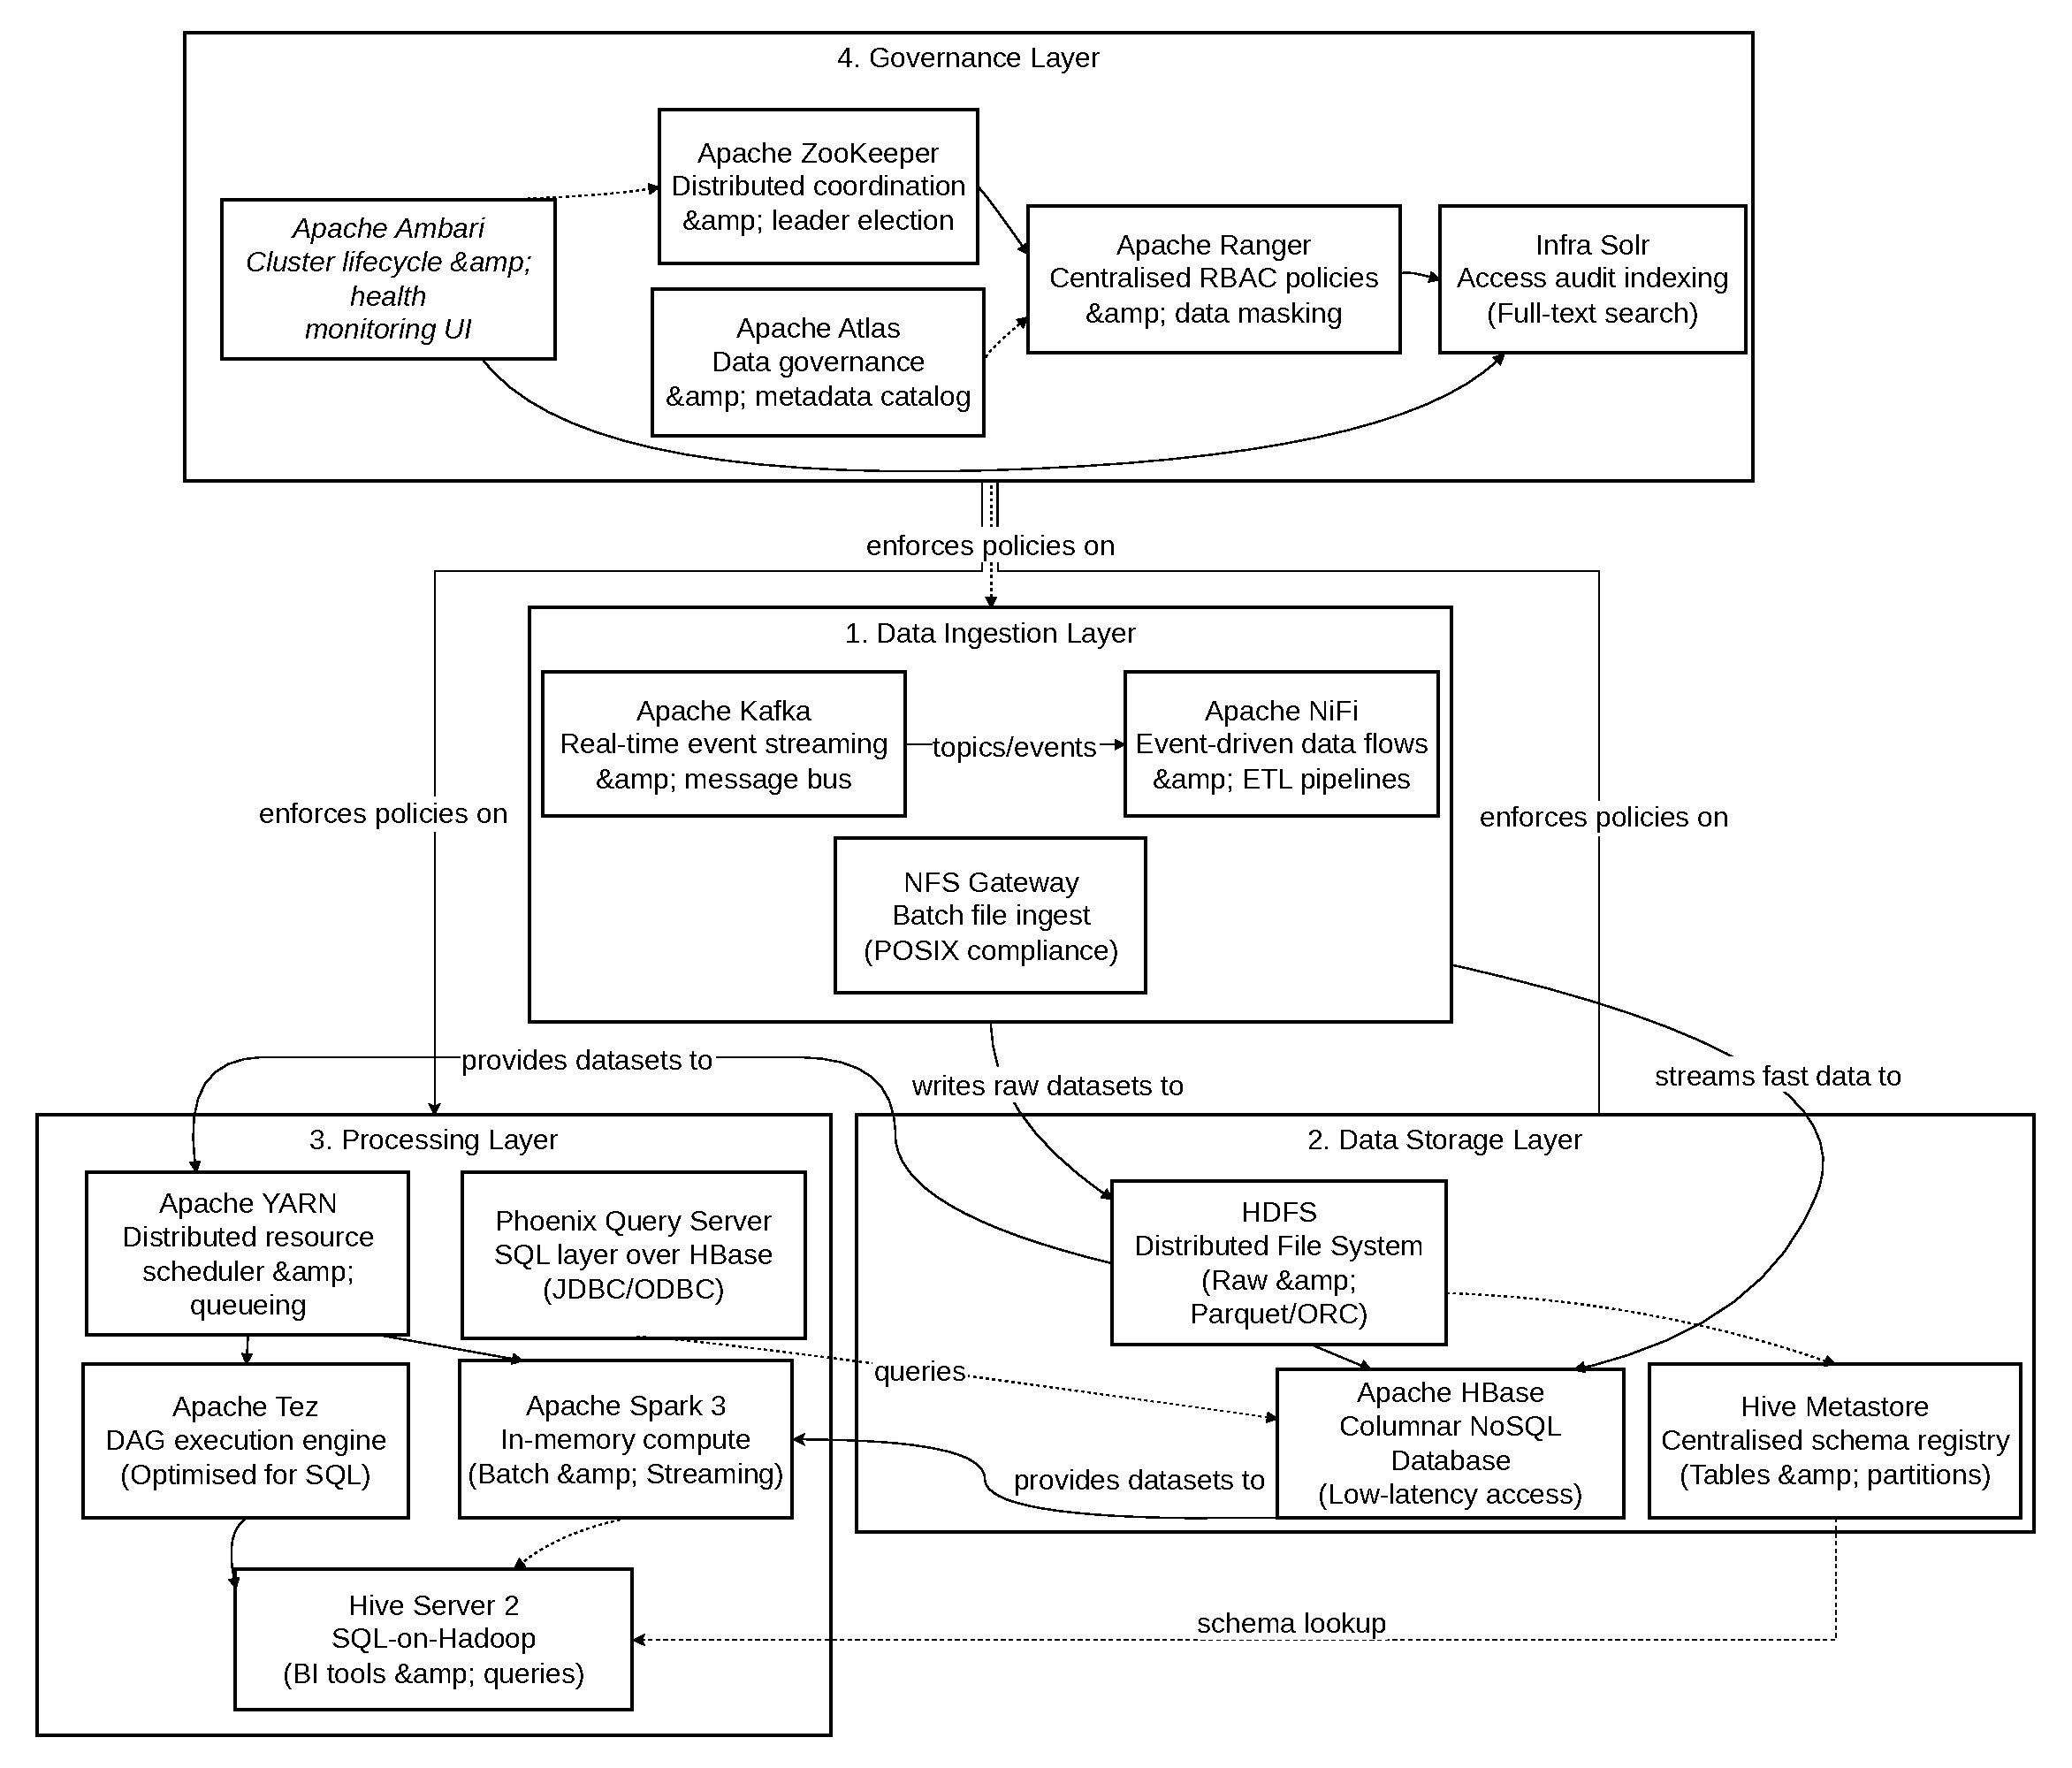
\includegraphics[width=\linewidth]{content/assets/datalake-architecture.pdf}
  \caption{Data Lake architecture, functional layers for the Default Profile.}
  \label{fig:arch-default}
\end{figure}

%%%%%%%%%%%%%%%%%%%%%%%%%%%%%%%%%%%%%%%%%%%%%%%%%%%%%%%%%%%%%%%%%%%%%%%%%%%%%%%%%%%%%%%%%%%%%%%%%%%%%%%%%%%%%%%%%%%
\subsection{Installation Profiles}

The framework supports three installation profiles, each deploying a different
subset of the architecture described above. The choice of profile is specified
as a Terraform variable before provisioning begins and determines which
components are distributed across the master and worker nodes during the
Ambari-driven deployment phase. This design allows the same IaC codebase to
serve distinct use cases without duplicating infrastructure definitions.

The \textbf{Default Profile} (Table~\ref{tab:comp-default}) installs the full
stack across all four layers, ingestion, storage, processing, and
governance, including NiFi, Kafka, HBase, Spark, Hive, and Ranger. It targets
environments that require end-to-end Data Lake functionality and serves as the
reference architecture against which the other profiles are derived.

The \textbf{Data Science Profile} (Table~\ref{tab:comp-data-science}) omits the
flow-based ingestion layer (NiFi) and the low-latency NoSQL tier (HBase,
Phoenix), concentrating cluster resources on Spark and Hive for analytical
processing and SQL-based workloads. By removing the memory and CPU overhead of
ingestion-oriented services, this profile frees resources for the in-memory
processing that Spark requires. It was used for the benchmark evaluation
reported in Section~\ref{sec:use-case}. Note that Kafka brokers remain in this
profile to support future streaming integration, although they were not
exercised during the benchmark.

The \textbf{Software Engineering Profile} retains NiFi, Kafka, HBase, and
Phoenix but excludes the analytical engines (Spark, Hive), reserving resources
for sustained event streaming, flow-based ingestion, and fast-retrieval
transactional operations.

\begin{table}[htbp]
  \centering
  \caption{Component mapping, Default Profile.}
  \label{tab:comp-default}
  \renewcommand{\arraystretch}{1.2}
  \begin{tabular}{@{} p{0.38\linewidth} p{0.58\linewidth} @{}}
    \hline
    \textbf{Node \& Role} & \textbf{Installed Components} \\
    \hline
    \textbf{master.cdp (10.0.0.2)} \newline \textit{Master Node} & Ambari Server, HBase Master, HistoryServer, NameNode, Phoenix Query Server, Ranger Admin, Ranger UserSync, ResourceManager, Secondary NameNode, Spark~3 JobHistoryServer, ZooKeeper Server \\
    \hline
    \textbf{node1.cdp (10.0.0.3)} \newline \textit{Worker Node~1} & DataNode, Hive Metastore, Hive Server, Kafka Broker, NFS Gateway, NiFi CA, NiFi Master, NodeManager, ZooKeeper Server \\
    \hline
    \textbf{node2.cdp (10.0.0.4)} \newline \textit{Worker Node~2} & DataNode, Kafka Broker, NodeManager, Spark~3 ThriftServer, ZooKeeper Server \\
    \hline
    \textbf{node3.cdp (10.0.0.5)} \newline \textit{Worker Node~3} & DataNode, HBase RegionServer, Kafka Broker, NodeManager, Ranger TagSync, Spark~3 Livy2 Server \\
    \hline
  \end{tabular}
\end{table}

\begin{table}[htbp]
  \centering
  \caption{Component mapping, Data Science Profile.}
  \label{tab:comp-data-science}
  \renewcommand{\arraystretch}{1.2}
  \begin{tabular}{@{} p{0.38\linewidth} p{0.58\linewidth} @{}}
    \hline
    \textbf{Node \& Role} & \textbf{Installed Components} \\
    \hline
    \textbf{master.cdp (10.0.0.2)} \newline \textit{Master Node} & HistoryServer, NameNode, Ranger Admin, Ranger UserSync, ResourceManager, Secondary NameNode, Spark~3 JobHistoryServer, ZooKeeper Server \\
    \hline
    \textbf{node1.cdp (10.0.0.3)} \newline \textit{Worker Node~1} & DataNode, Hive Metastore, Hive Server, Kafka Broker, NFS Gateway, NodeManager, ZooKeeper Server \\
    \hline
    \textbf{node2.cdp (10.0.0.4)} \newline \textit{Worker Node~2} & DataNode, Kafka Broker, NodeManager, Spark~3 ThriftServer, ZooKeeper Server \\
    \hline
    \textbf{node3.cdp (10.0.0.5)} \newline \textit{Worker Node~3} & DataNode, Kafka Broker, NodeManager, Ranger TagSync, Spark~3 Livy2 Server \\
    \hline
  \end{tabular}
\end{table}
